\documentclass[12pt, a4paper]{article}
\usepackage[utf8]{inputenc}
\usepackage{graphicx}

% Update this information to reflect yourself
\title{Assignment 1: 3SUM}
\author{Georgios Rounis}
\date{2022-09-19}

\begin{document}
\maketitle

\section{Introduction}

The current report aims to present the results of the experiments that compare the performance of different algorithms used to solve the 3SUM and the 4SUM problem. In addition, for each implementation, a set of unit tests has been created to verify the given solution and ensure the validity of each algorithm. Lastly, the results are presented numerically in a table and visually as a plot. Please find the code in the following repo path:
\textit{https://github.itu.dk/gero/ThreeFourSum2022.git}

\section{Implementation}
\subsection{3SUM}
The 3SUM problem includes a common cubic algorithm with three nested loops, a quadratic algorithm that initially sorts the input list, and through a smart linear read, we discover if there are values that satisfy our conditions. The last algorithm describes a more sophisticated solution that stores all the elements of the list in a hash map, along with their indices in the original list, and iterates over each pair of elements (a,b) till we find a value equal to $-a - b$ that is in the list. The reason why there is an additional check for $j < k$ is to ensure that each value on the list is not used more than once.

\subsection{4SUM}
The first solution for 4SUM is the try of all elements (4 nested for loops) that ensures a quartic running time. Like in 3SUM, the alternative solution(cubic) sorts the list and performs a specific sequential search. The running time of this solution is cubic. The last algorithm stores in a hash-map, the sum of a + b together with a list of tuples (a, b).

\subsection{Unit Testing}
To verify the correctness of the implementations a set of test cases using assertNull, assertNotNull and assertArrayEquals methods have been created, using JUnit.


\section{Experiments}

After the algorithms implementation and the extensive unit testing, the project was built as two JAR packages(one for 3SUM and 4SUM respectively) producing the expected output along with the main method. The algorithms have been called from Python and NumPy was used to generate random
input. A measurement function has been added in order to measure the
running time of the specified algorithm. After implementing individual
measurements, the framework to perform a set of experiments was included, and which creates a .csv file for the results of either 4SUM or 3SUM (depends on which algorithm you invoke). The data are presented numerically in tables which include the Average running time and the Standard deviation in relation to the number n of items. Then plots for our algorithms have been created using the refined results.

\section{Results}

Looking at the results of 3SUM problem experiments, we conclude that The three implementations have a similar running time when the input is small. As the number of elements n increases, the running time increases dramatically. It is clear according to the plot that the Quadratic implementation performs better than the Hash-map solution (for n=577536 hashmap solutions has almost the same running time with quadratic for n =227414) while theoretically both should be quadratic worst case. We assume this happens due to Java implementation of Hashmap.

\begin{table}[h]
  \begin{center}
  \caption{With a \textbf{TIMEOUT = 30}, \textbf{I MAX value = 30} and \textbf{M = 5}. 
  Cubic average worst-case running time for 3SUM problem.}
  \label{tbl:threesum_cubic}
  \begin{tabular}{rrr}
$n$ & Average (s) & Standard deviation (s) \\\hline
30 & 0.140171 & 0.010673\\ 
42 & 0.146144 & 0.020116\\ 
59 & 0.141777 & 0.018397\\ 
84 & 0.129918 & 0.005950\\ 
118 & 0.148018 & 0.003106\\ 
167 & 0.152478 & 0.014500\\ 
235 & 0.152015 & 0.005566\\ 
332 & 0.141965 & 0.004402\\ 
468 & 0.147808 & 0.011707\\ 
660 & 0.160089 & 0.001407\\ 
931 & 0.193085 & 0.013436\\ 
1313 & 0.273100 & 0.012939\\ 
1852 & 0.461591 & 0.007888\\ 
2611 & 1.015820 & 0.020648\\ 
3682 & 2.518729 & 0.018326\\ 
5192 & 6.860553 & 0.142883\\ 
7321 & 18.351312 & 0.049254\\ 
\end{tabular}

  \end{center}
\end{table}

\begin{table}[h]
  \begin{center}
  \caption{With a \textbf{TIMEOUT = 30}, \textbf{I MAX value = 30} and \textbf{M = 5}. 
  Quadratic average worst-case running time for 3SUM problem.}
  \label{tbl:threesum_quadratic}
  \begin{tabular}{rrr}
$n$ & Average (s) & Standard deviation (s) \\\hline
30 & 0.143809 & 0.014019\\ 
42 & 0.132696 & 0.006331\\ 
59 & 0.132097 & 0.009521\\ 
84 & 0.132003 & 0.007655\\ 
118 & 0.136862 & 0.006938\\ 
167 & 0.134091 & 0.006119\\ 
235 & 0.133052 & 0.004961\\ 
332 & 0.154633 & 0.003422\\ 
468 & 0.146676 & 0.012018\\ 
660 & 0.163840 & 0.006727\\ 
931 & 0.163946 & 0.005326\\ 
1313 & 0.172590 & 0.018674\\ 
1852 & 0.164984 & 0.005305\\ 
2611 & 0.197714 & 0.034761\\ 
3682 & 0.187579 & 0.020836\\ 
5192 & 0.176480 & 0.002790\\ 
7321 & 0.199638 & 0.004680\\ 
10323 & 0.242216 & 0.019688\\ 
14556 & 0.272198 & 0.009067\\ 
20525 & 0.403532 & 0.032526\\ 
28940 & 0.522313 & 0.007790\\ 
40805 & 0.873079 & 0.041449\\ 
57536 & 1.490500 & 0.029636\\ 
81126 & 2.717598 & 0.040837\\ 
114387 & 5.164560 & 0.028166\\ 
161286 & 10.079573 & 0.069456\\ 
227414 & 19.763368 & 0.018043\\ 
\end{tabular}

  \end{center}
\end{table}

\begin{table}[h]
  \begin{center}
  \caption{With a \textbf{TIMEOUT = 30}, \textbf{I MAX value = 30} and \textbf{M = 5}. 
  Hashmap average worst-case running time for 3SUM problem.}
  \label{tbl:threesum_hashmap}
  \begin{tabular}{rrr}
$n$ & Average (s) & Standard deviation (s) \\\hline
30 & 0.128695 & 0.005329\\ 
42 & 0.131030 & 0.007553\\ 
59 & 0.134144 & 0.006554\\ 
84 & 0.130913 & 0.006966\\ 
118 & 0.156230 & 0.010406\\ 
167 & 0.156671 & 0.013668\\ 
235 & 0.148050 & 0.005151\\ 
332 & 0.147941 & 0.009732\\ 
468 & 0.144672 & 0.008125\\ 
660 & 0.173362 & 0.004388\\ 
931 & 0.153885 & 0.006247\\ 
1313 & 0.163004 & 0.003845\\ 
1852 & 0.179052 & 0.007044\\ 
2611 & 0.209766 & 0.016319\\ 
3682 & 0.245553 & 0.005238\\ 
5192 & 0.367003 & 0.011408\\ 
7321 & 0.700999 & 0.160194\\ 
10323 & 0.980280 & 0.089060\\ 
14556 & 1.391312 & 0.038462\\ 
20525 & 3.049984 & 0.063293\\ 
28940 & 5.102823 & 0.202491\\ 
40805 & 11.853841 & 0.141200\\ 
57536 & 20.298086 & 0.156000\\ 
\end{tabular}

  \end{center}
\end{table}

\begin{figure}[h]
  \begin{center}
    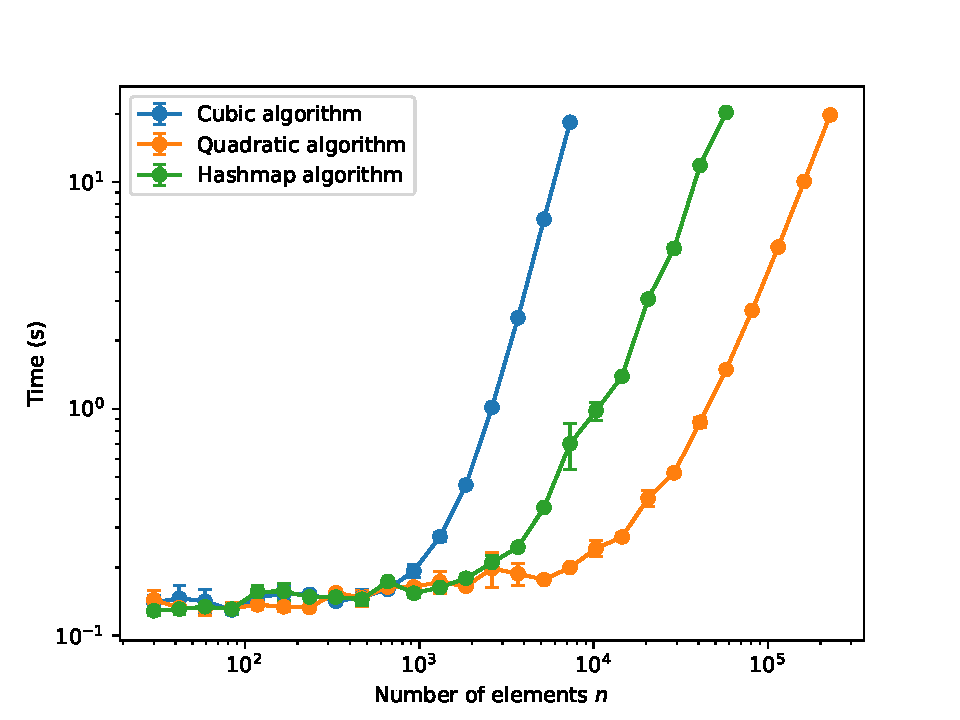
\includegraphics[width=\textwidth]{Plot_threesum.pdf}
    \caption{Plot showing the running times of 3SUM problem}
    \label{fig:plot3sum}
  \end{center}
\end{figure}

\clearpage

According to the results of the 4SUM problem, we conclude that all three solutions perform similar when the number of element n is small, but Hashmap solution performs the best as the number n is increased, slightly better than the cubic one.

\begin{table}[h]
  \begin{center}
  \caption{With a \textbf{TIMEOUT = 30}, \textbf{I MAX value = 30} and \textbf{M = 5}. 
  Quartic average worst-case running time for 4SUM problem.}
  \label{tbl:threesum_quadratic}
  \input{foursum_quartic_tabular.tex}
  \end{center}
\end{table}

\begin{table}[h]
  \begin{center}
  \caption{With a \textbf{TIMEOUT = 30}, \textbf{I MAX value = 30} and \textbf{M = 5}. 
  Cubic average worst-case running time for 4SUM problem.}
  \label{tbl:foursum_cubic}
  \input{foursum_cubic_tabular.tex}
  \end{center}
\end{table}

\begin{table}[h]
  \begin{center}
  \caption{With a \textbf{TIMEOUT = 30}, \textbf{I MAX value = 30} and \textbf{M = 5}. 
  Hashmap average worst-case running time for 4SUM problem.}
  \label{tbl:foursum_hashmap}
  \input{foursum_hashmap_tabular.tex}
  \end{center}
\end{table}

\begin{figure}[h]
  \begin{center}
    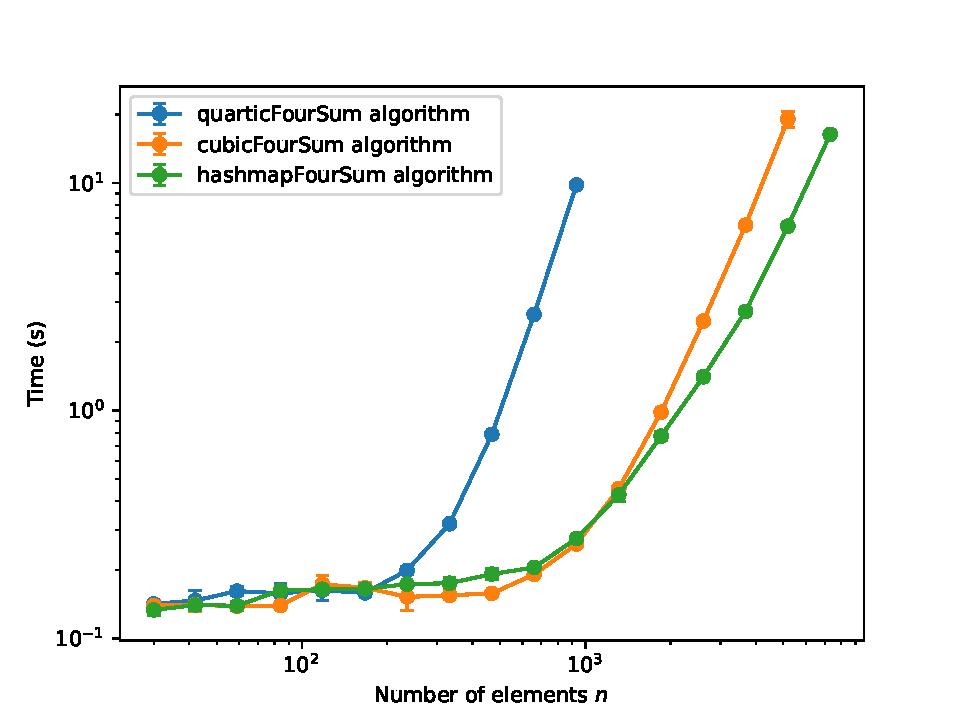
\includegraphics[width=\textwidth]{Plot_foursum.pdf}
    \caption{Plot showing the running times of 4SUM problem}
    \label{fig:plot3sum}
  \end{center}
\end{figure}

\clearpage
\end{document}

